%% Appendix
\appendix

\section{Additional NS Examples}
\label{appendix:MoreNsExamples}



\subsection{Motivating Examples \#1}
\label{appendix:subsec::Ex1A:NS}


Recall the code snipped from Listing~\ref{lst:MotivatingExample1Ser}:


\begin{minipage}[t]{0.3\textwidth}
	\begin{lstlisting}[caption={Without yield or lock (serializable)}]
	request main: 
		X := 1 
		// no yield
		y := X 
		X := 0
		return y 
	\end{lstlisting}
\end{minipage}

\begin{figure}[htbp]
	\centering
	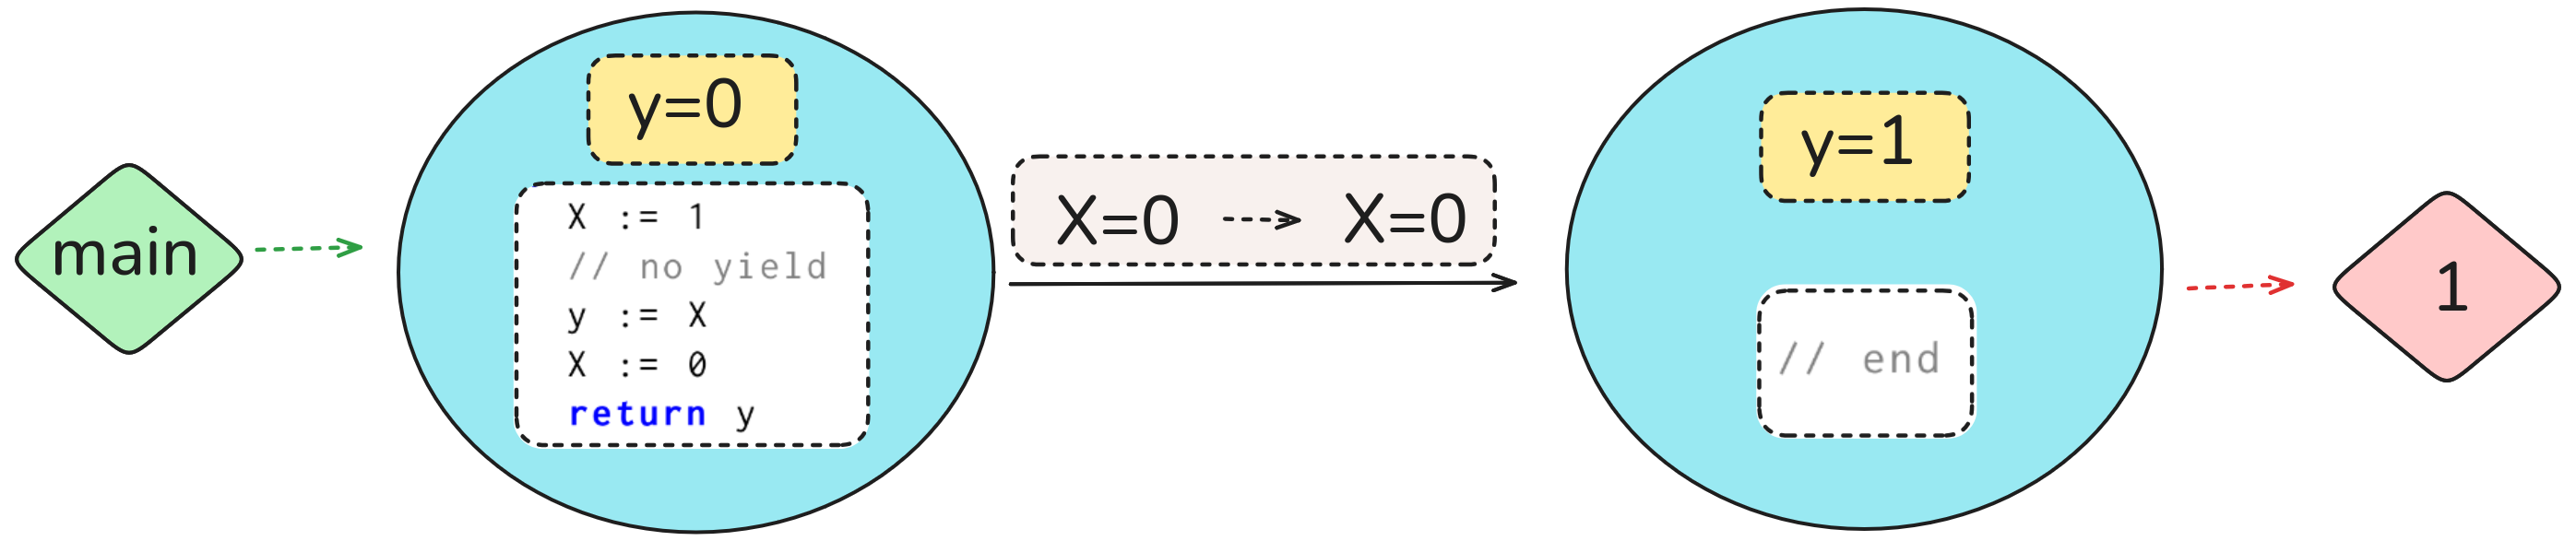
\includegraphics[width=0.9\textwidth]{plots/code_1_NS.png}
	\caption{Network System for interleaving executions of Listing~\ref{lst:MotivatingExample1Ser} program.}
	\label{fig:code1ExampleNS}
\end{figure}


\begin{figure}[htbp]
	\centering
	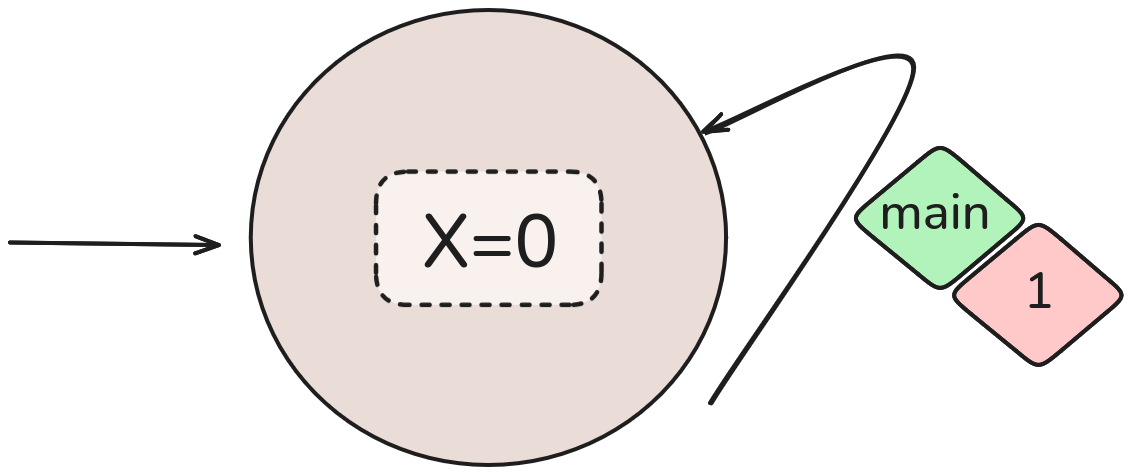
\includegraphics[width=0.35\textwidth]{plots/code_1_NFA.png}
	\caption{NFA for serialized executions of Listing~\ref{lst:MotivatingExample1Ser} program.}
	\label{fig:code1ExampleNFA}
\end{figure}



\begin{figure}[htbp]
	\centering
	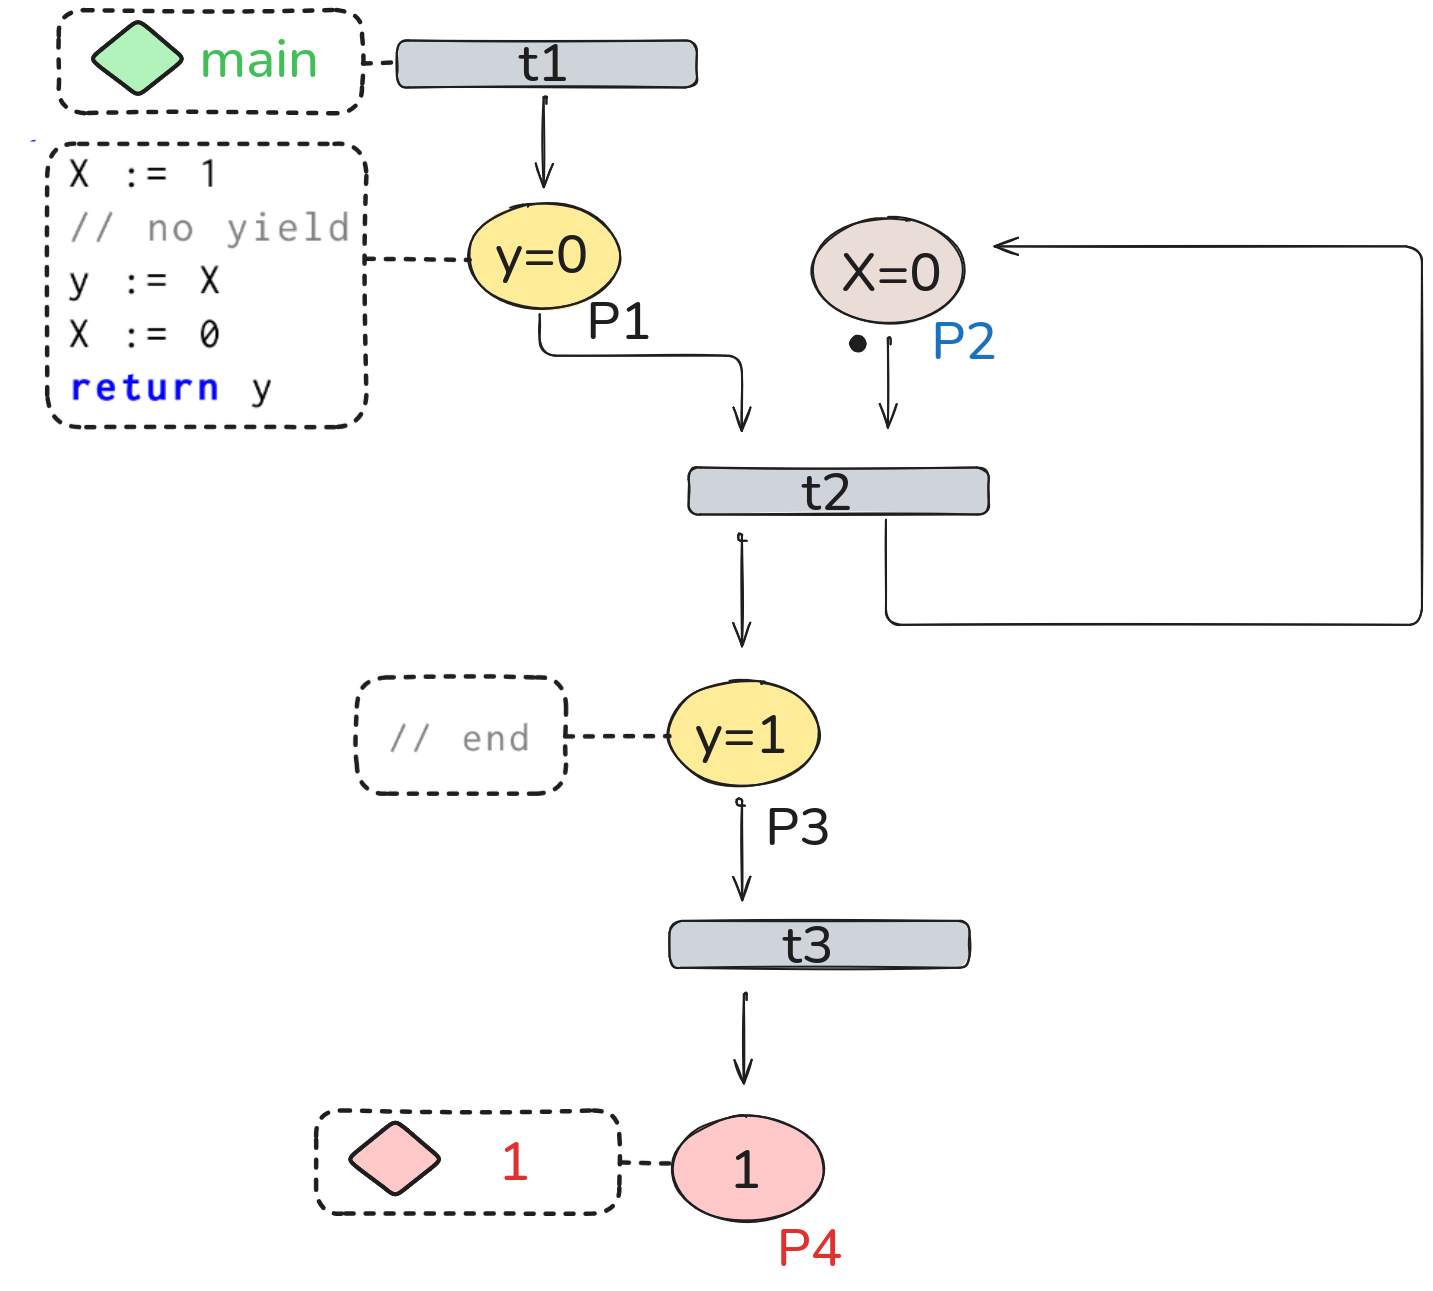
\includegraphics[width=0.6\textwidth]{plots/code_1_PN_with_annotation.png}
	\caption{Petri Net for interleaving executions of Listing~\ref{lst:MotivatingExample1Ser} program.}
	\label{fig:code1ExamplePN}
\end{figure}

%

\subsection{Motivating Examples \#2}
\label{appendix:subsec::Ex1B:NS}

For details, see the main text (Sec.~\ref{sec:problem-definition}).


\subsection{Motivating Examples \#3}
\label{appendix:subsec:Ex1C:NS}

Recall our third motivating example, presented in Listing~\ref{lst:MotivatingExample3SerAgain}.

\begin{minipage}[t]{0.3\textwidth}
	\begin{lstlisting}[caption={With yield and lock (serializable)}]
		request foo: 
			// lock
			while (L == 1): 
				yield
			L := 1 
		
			X := 1
			yield
			y := X 
			X := 0
		
			// unlock    
			L := 0
			return y 
	\end{lstlisting}
\end{minipage}

This program corresponds to the following Network System (NS):

\begin{figure}[htbp]
	\centering
	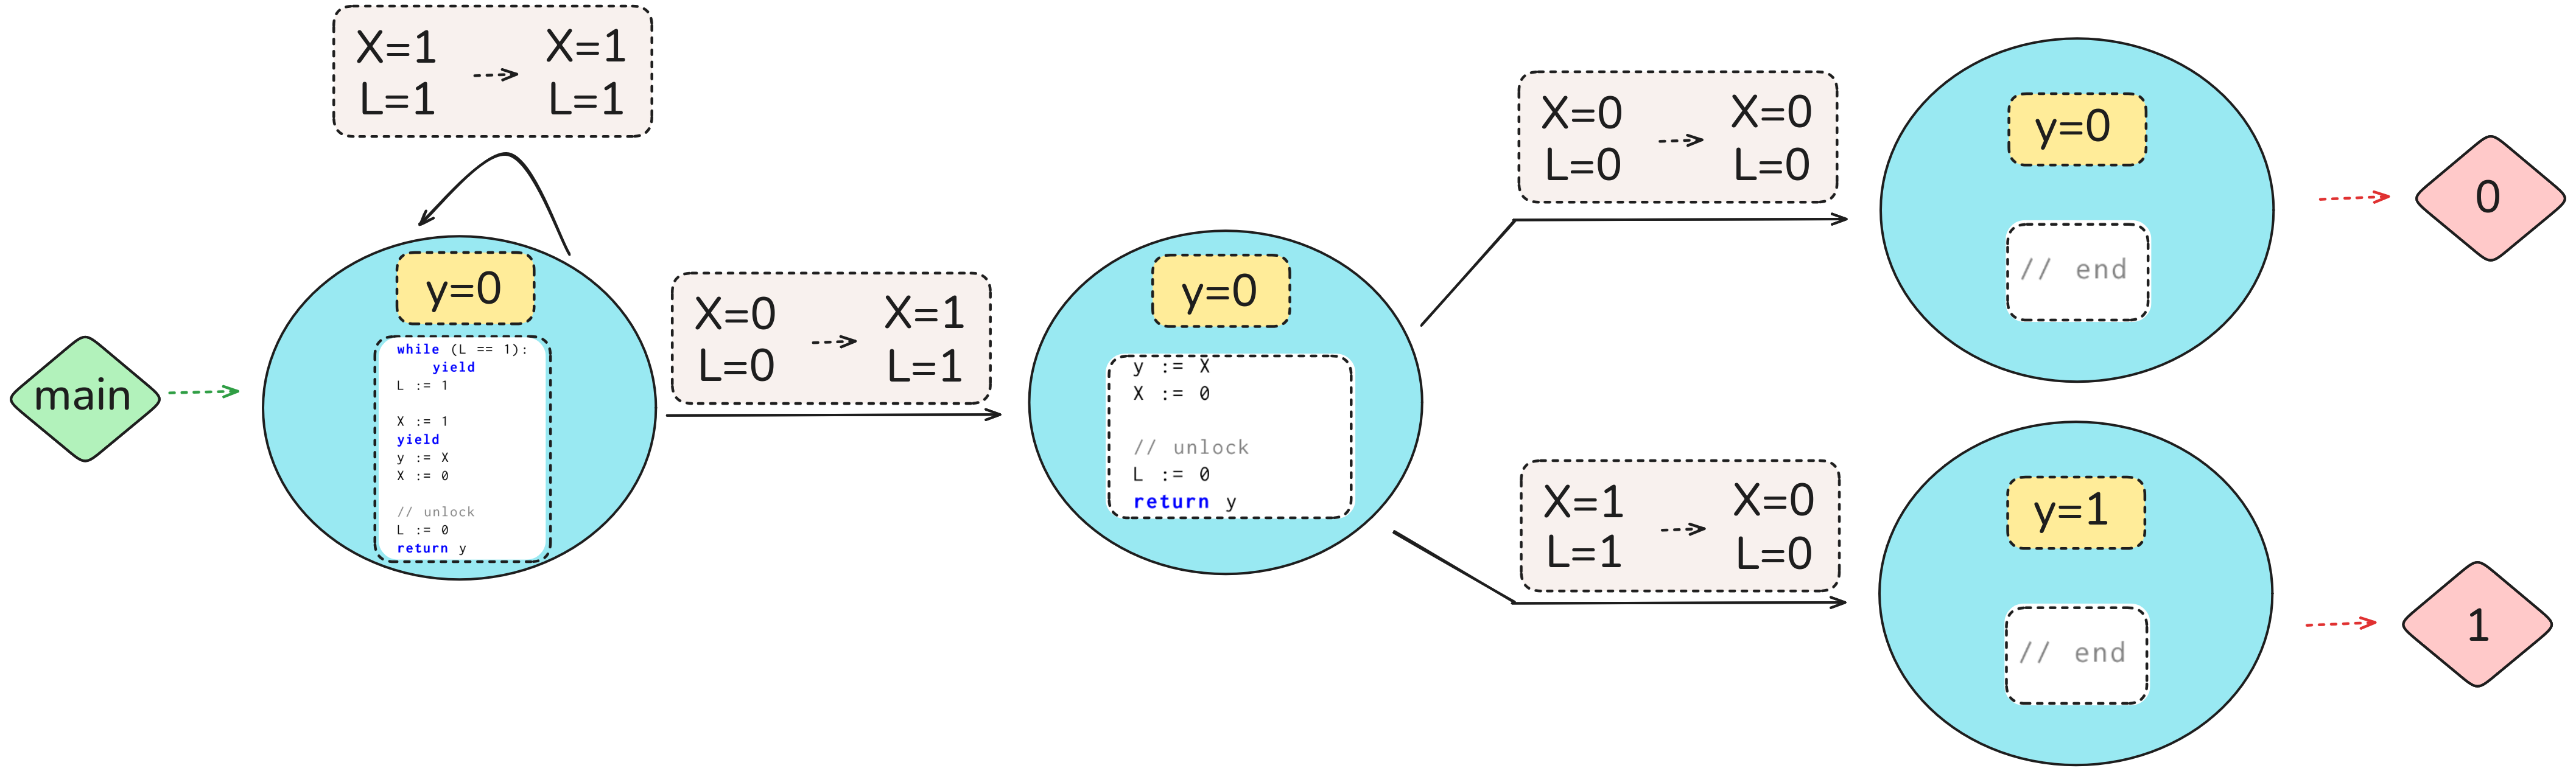
\includegraphics[width=1.1\textwidth]{plots/code_3_NS.png}
	\caption{Network System for interleaving executions of Listing~\ref{lst:MotivatingExample3Ser} program.}
	\label{fig:code3ExampleNS}
\end{figure}


\begin{figure}[htbp]
	\centering
	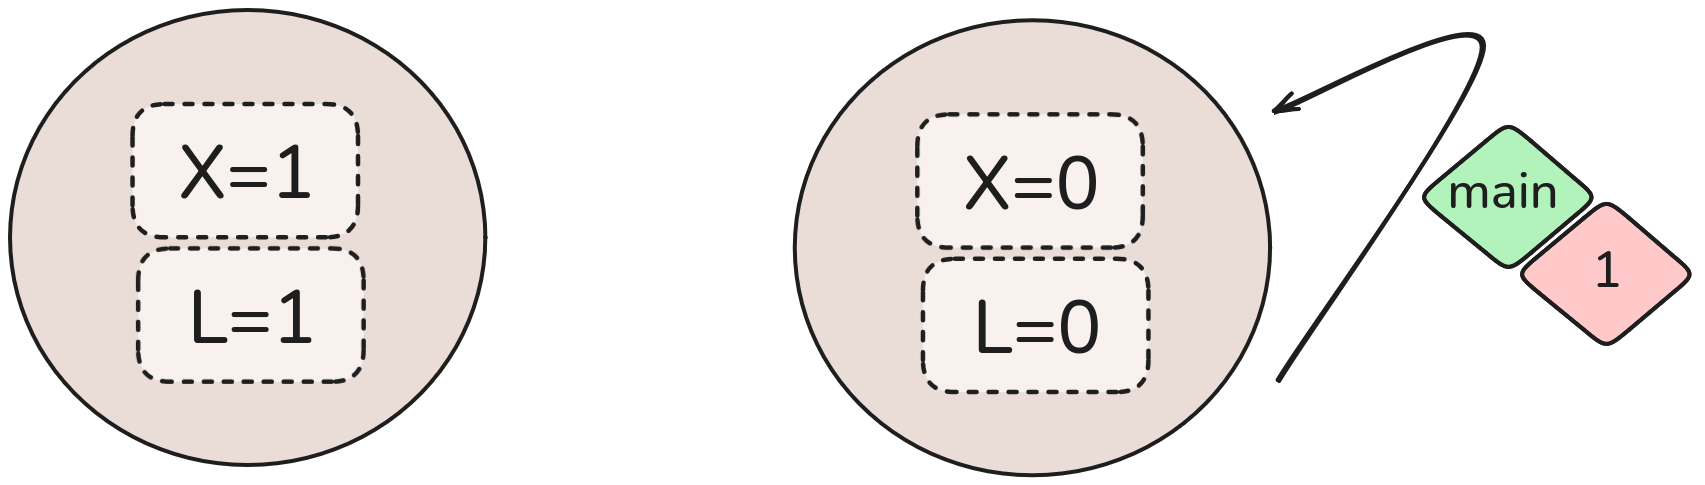
\includegraphics[width=0.4\textwidth]{plots/code_3_NFA.png}
	\caption{NFA for serialized executions of Listing~\ref{lst:MotivatingExample3Ser} program.}
	\label{fig:code3ExampleNFA}
\end{figure}



\begin{figure}[H]
	\centering
	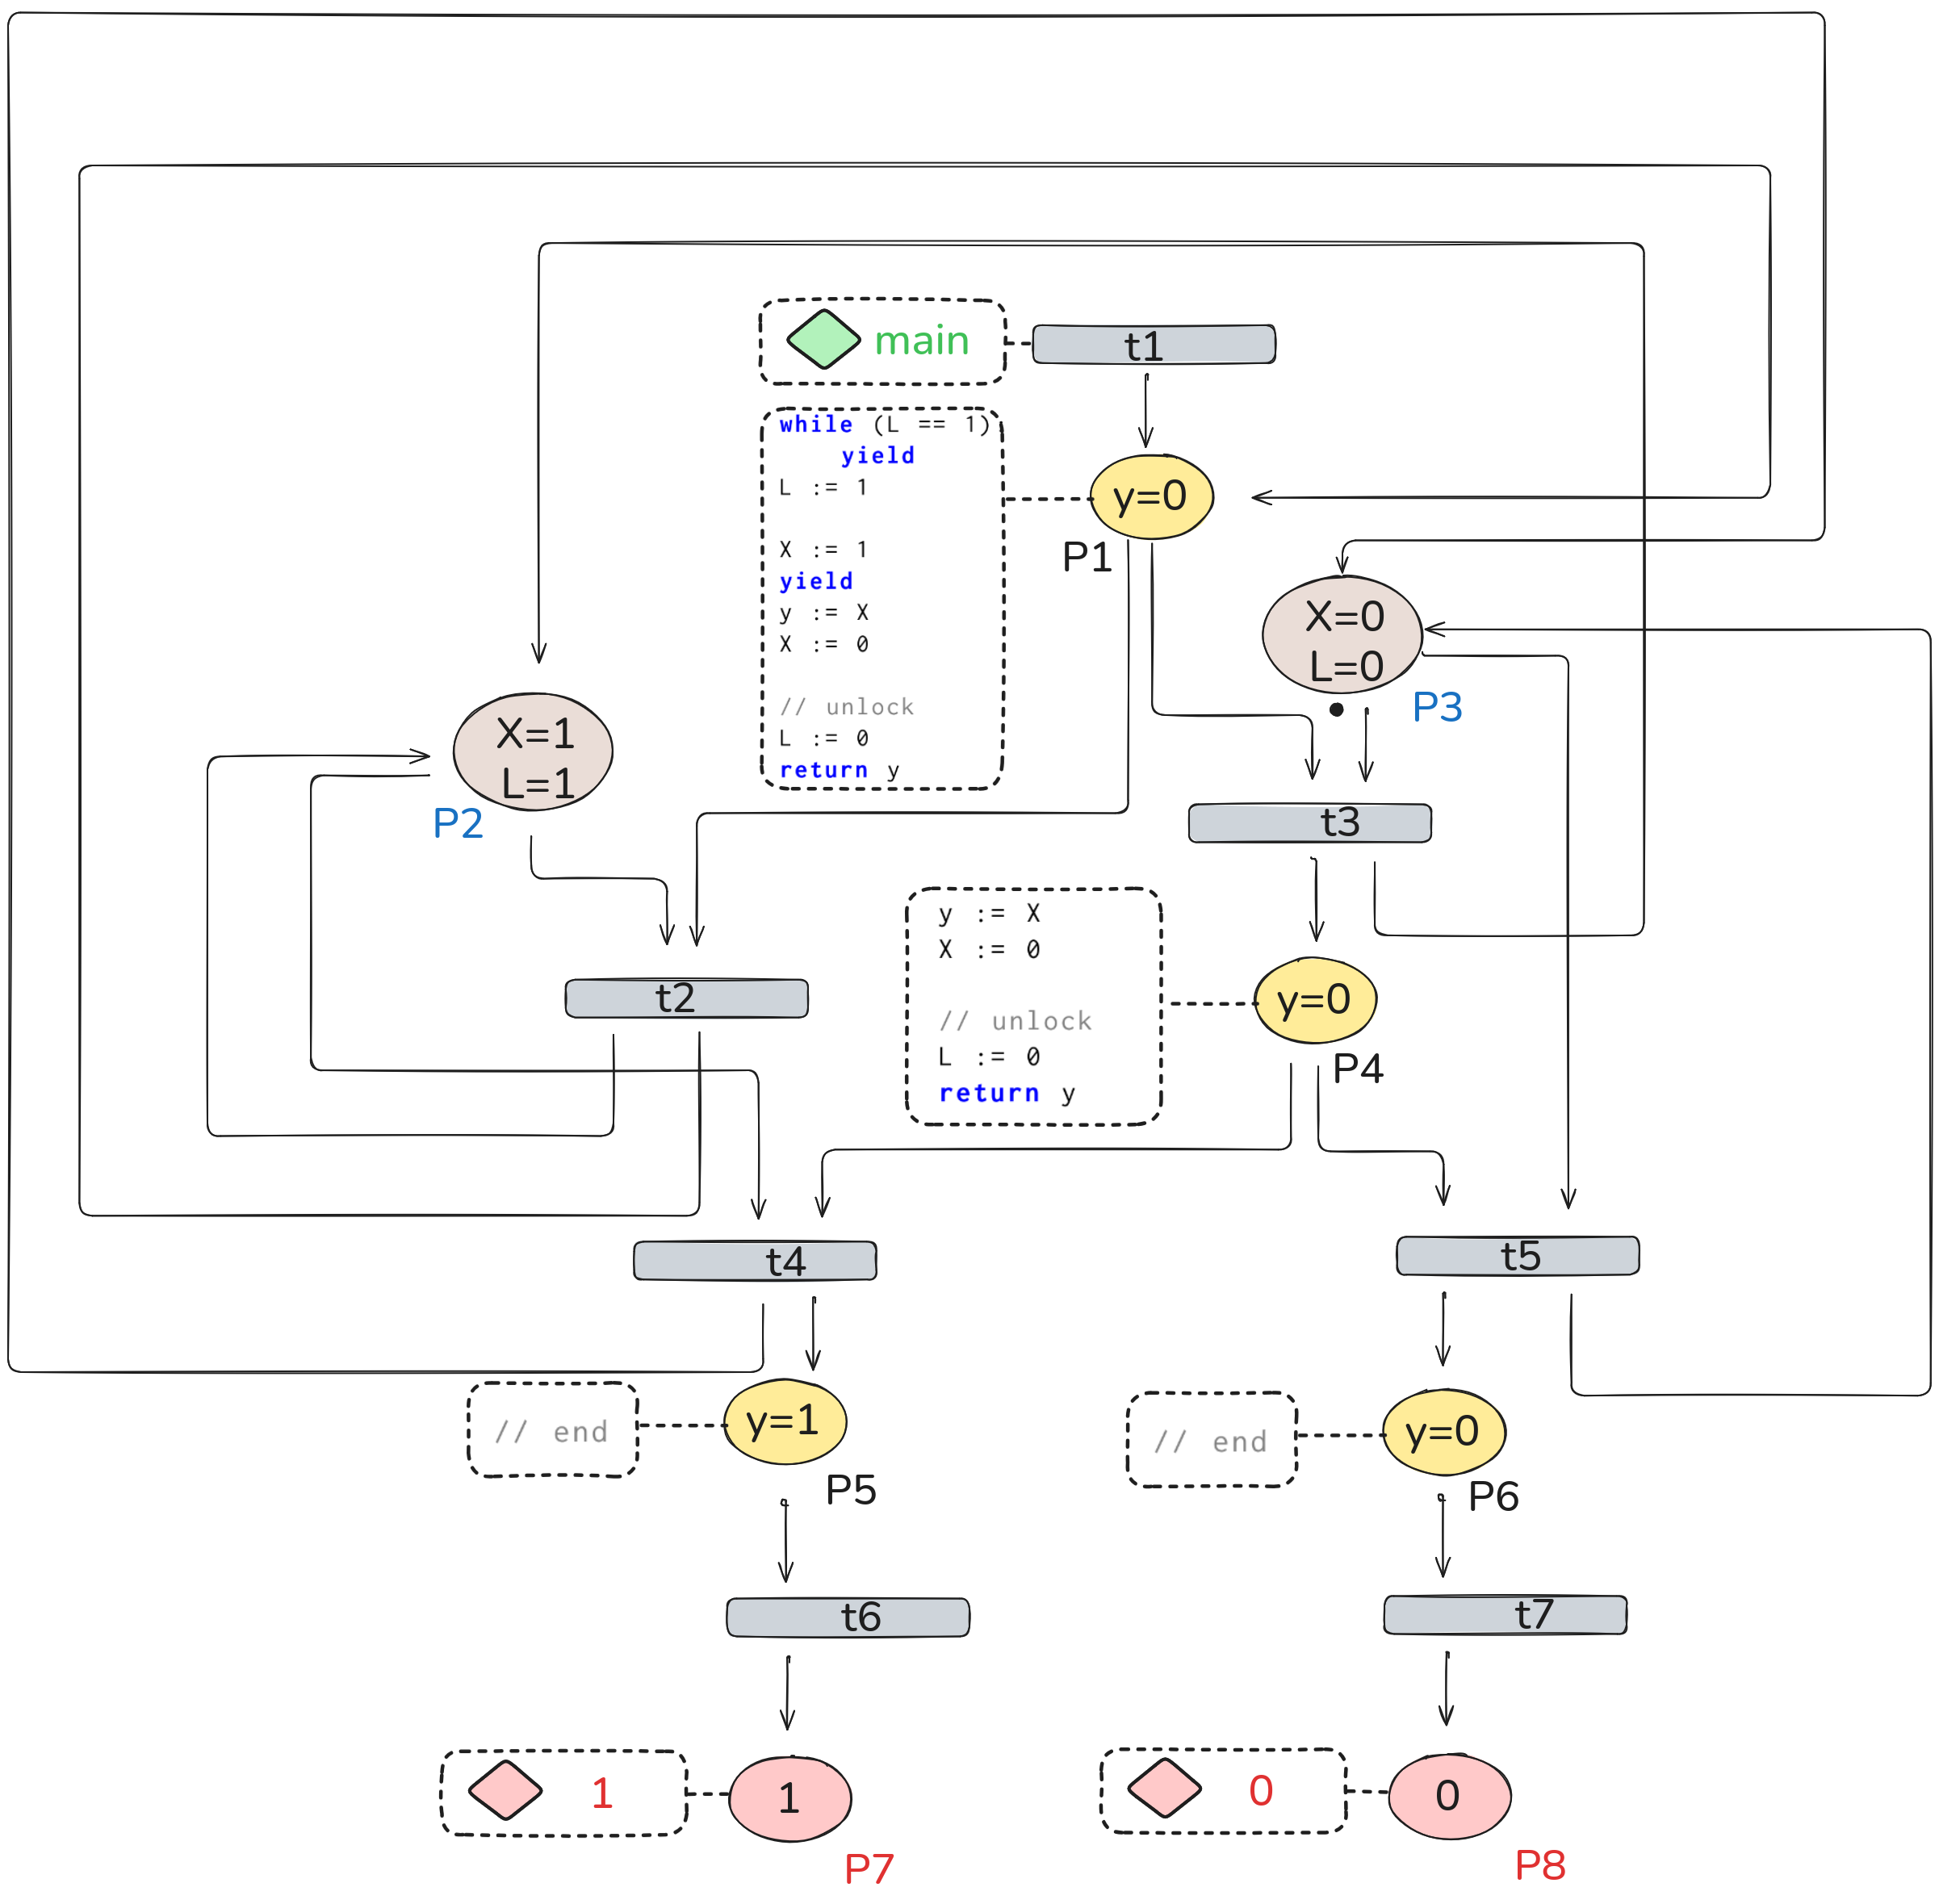
\includegraphics[width=0.8\textwidth]{plots/code_3_PN_with_annotation.png}
	\caption{Petri Net for interleaving executions of Listing~\ref{lst:MotivatingExample3Ser} program.}
	\label{fig:code3ExamplePN}
\end{figure}

\newpage